\documentclass[12pt,a4paper]{article}
\usepackage{fullpage}
\usepackage[utf8]{inputenc}
\usepackage{indentfirst}

\usepackage{graphicx}
\graphicspath{ {./img/} }


\usepackage[hidelinks]{hyperref}
\usepackage{float}


\let\oldsection\section
\renewcommand\section{\clearpage\oldsection}

\newcommand{\dofigure}[3][H]{
    \begin{figure}[#1]
        \centering
        \includegraphics[width=\textwidth]{#2}
        \caption{#3}
    \end{figure}
}

\begin{document}
    \begin{titlepage}
        \begin{center}
            {\Huge \textbf {Enhanced Pong}}

            \vspace{0.5cm}
            {\LARGE Digital platforms project B}

            \vspace{1.5cm}
            Merzlyakov Ilya, Batenko Nikita, Feshchenko Igor

            \vfill
            Novosibirsk State University \\
            2021

        \end{center}
    \end{titlepage}
    \tableofcontents
    \section{Introduction and work description}

    This documentation have been made for describing contents of our semester project “The game of TV-Tennis”.  This game were invented in 1969 by Ralph Baering and was called “The Game of Pong”. It were played by specific controller with two joysticks for two people on the one of the first TV model “Brown Box”. In our game would be only one human player and the second one would an artificial intelligence.

    Used programs and developing tools: Logisim v.2.7.1, CocoIDE v.1.91, PythonIDE v.3.8, Java 11.

    Our reasons of taking this project:
    \begin{itemize}
        \item We found most interesting of all three. The most attractive part of it is that it uses one comparatively big pixel display and joystick instead of buttons like in projects A and B.
        \item It is middle difficulty in realization. When we were on stage of choosing, it was not so primitively looking like “The Game of Noughts and Crosses” and not as hard as “The Game of Mancala”. 
    \end{itemize}
    The next step was to determine roles in our project. Our roles:
    \begin{itemize}
        \item Merzlyakov Ilya – made whole artificial intelligence and scripts of uploading images, took part in designing digital scheme by making ball moving computation
        \item Batenko Nikita – took part in making video system (video chips, video decoder and score counting), has written documentation and drew most of pictures for the game
        \item Feshchenko Igor – in cooperation with Ilya made kinematic controller and system of writing and reading data to/from memory, took major part in designing digital scheme
    \end{itemize}
    he contribution in our project of each teammate has divided like this: 
    Ilya Merzlyakov – about 40\%, Batenko Nikita – 30\%, Feshchenko Igor 30\%.
    \subsection{Our main goal}
    Make playable game with nice looking intro and outros for winning and losing. The ball movement trajectory is simple which computes for constant angles (± 30°) and simple AI, which reacts on changing sign of ball angle. The computer can only move its bat while the ball is in the left-hand half of the screen (the human player’s half). As soon as the ball enters the right-hand half, the game controller (kinematic controller) blocks the right bat.

    We have completed minimum goal for about 5-6 weeks and continued expand project by extensions that will be described next.

    \subsection{Extensions}
    The first extension we made is a start/restart button. It allows restarting the whole game to the beginning (excluding introduction). It resets scores to zero, resets ball and bats positions.

    The second additional goal was harder. We decided to make game more interesting by improving ball movement angles. We made more complex angle system, which allows ball to move not only straight and by diagonal of two angles (30° or 150°), but using 256 angles in range from $-{\pi\over4}$ to $\pi\over4$. Sometimes it leads ball to move in hardly predictable ways.

    However, such way of computing ball movement requires of better artificial intelligence, which must predict balls trajectory. It uses a little bit more math formulas for it comparing to base version, which determines bats behavior mostly by sign of coordinates of ball. Now, we work on it.

    And the last, but not the least improvement is graphical. We made an algorithm, which shows introduction pictures, winning and losing screens in appropriate situations (beginning playing, winning AI or losing to it).

    \subsection{Working process and problems}
    We had not have a concrete plan of work, but now all working progress can be divided on the following points:
    \begin{enumerate}
        \item Choose and build convenient system architecture
        \item Connect memory and processor to display\begin{enumerate}
            \item Make video chips
            \item Connect video chips to display
            \item Connect memory and processor to video system
        \end{enumerate}
        \item Write kinematic controller\begin{enumerate}
            \item Write inner chips for kinematic
            \item Make kinematic controller systems
        \end{enumerate}
        \item Connect kinematic controller to video system
        \item Make and connect scoring system
        \item Write base AI and make appropriate connections to processor and main memory (RAM)
        \item Make restart button
        \item Make “cut scenes” addition\begin{enumerate}
            \item Draw pictures
            \item Write Python encoding program
            \item Make decoder scheme
            \item Connect decoder to video system and add conditions of launching
        \end{enumerate}
        \item Upgrade trajectory-computing system \begin{enumerate}
            \item Add RAMs containing trigonometric representations of angles to kinematic controller
            \item Upgrade velocity and angles computing sub-schemes of kinematic controller
        \end{enumerate}
        \item Improve AI
        \item Rearrange scheme for nicer looking, add more commentaries to code
        \item Write documentation
    \end{enumerate}

    During the work, we have faced the problem of regular reuploading of our memory images for AI, images and angles table into Logisim after refreshing the project. To save some time and make work less routine Ilya has wrote a Java script, which automatically loads memory images, when it is needed. It is out of our project and this script is not described here.

    At this point, the introduction ends and begins the description of project. It splits on two big parts:
    \begin{itemize}
        \item Description of digital scheme of our project
        \item Description of game artificial intelligence and its working principle
    \end{itemize}


    \section{Digital scheme}
    Before jumping into details, the whole system plan must be introduced. It is hard to show whole scheme directly, because in that case there would be too much little and hardly readable details. Here is an oversimplified plan of our blueprint (Picture 1). In the next sections of documentation, more circuits that are detailed would be shown. In this you can see a division of our project on modules and how they interact with each other.
    \dofigure{scheme.png}{Oversimplified plan of digital scheme}

    The contents of scheme:
    \begin{itemize}
        \item The Player interface part consists of 32x32 pixels display and number indicators, which show the current score of human player and bot.
        \item Video chips is a pack of 4 connected video sections, each of which consists of 8 video chips connected to each other. There are 32 video chips in total for every column of display pixels.
        \item Kinematic controller is a complex pack of partly independent circuits including angle and velocity computation chips. Whole module computes angle and velocity of ball; detects and computes hitting of walls and bats; updates scores.
        \item Video player exists for only one purpose – to show intro, winning and losing screens, when specific conditions fulfilled.
        \item The block with start/restart button and joystick is a part of user interface too. They are used to launch or restart the game and to control the left bat.
        \item Game conditions block is used to execute video player and end game, when winning or losing conditions are fulfilled.
        \item The CdM-8 (mark 5) processor – the heart of the whole digital scheme. Used to execute program code, which can be taken from memory block.
        \item Data reading/writing block is a sequence of 14 similar circuits, which read and write data from/to registers of processor and give it to Kinematic controller module, Operations accelerator module.
        \item  Operations accelerator – the module, which accelerates division and multiplication operations for processor. Helps to compute ball trajectory.
        \item Memory consists of RAM, which contains program with AI for right bat.
    \end{itemize}

    As you can see, Data reading/writing block, Operation accelerator, Processor and memory are combined together in one AI block.

    The best frequencies to play the game are 256Hz or 512Hz. On these frequencies, the ball will have such speed that it would be a challenge for human to reflect it with bat and not too fast, that AI would be unbeatable. 

    \subsection{Video chips}
    Video systems consists of two parts: video chips and video player. We will start with video chips. As were said, video chips are combined in 4 blocks with 8 chips in each – 32 chips in total. 

    % \begin{figure}[h]
    %     \centering
    %     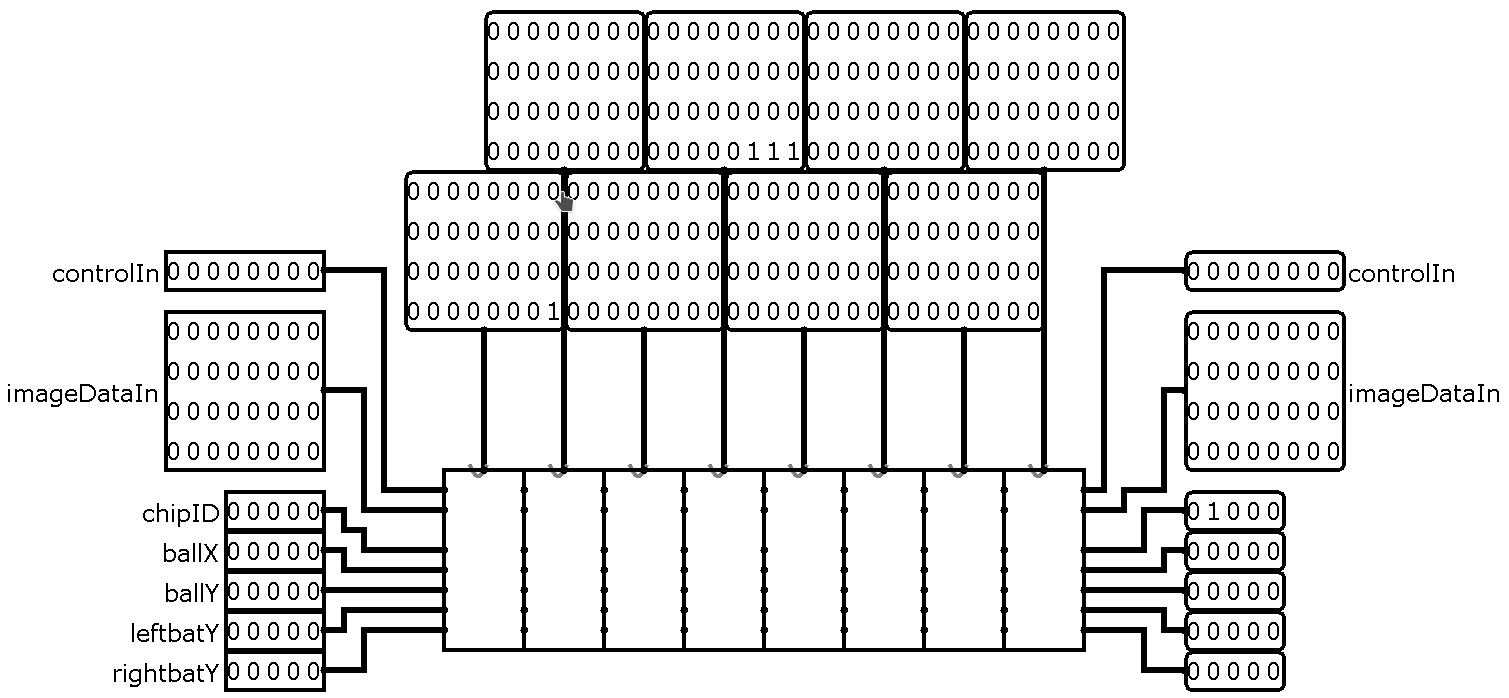
\includegraphics[width=\textwidth]{video_section.png}
    %     \caption{Video section}
    % \end{figure}
    \dofigure{video_section.png}{Video Section}
    Every video section and every chip inside them receive five 5-bit numbers: ballX and ballY – coordinates of ball, leftbatX and leftbatY – coordinates of bats and chipID – the unique ID of every chip and column of 32 pixels to which it connects.
    \dofigure{video_chip.png}{Video chip}

    Inner circuit is just a decoder which only activates when chipID matches specified constant.

    As you can see in Picture 3, if some chip should show the left or right bat, its coordinates are combined with the similar but moved on 1 and 2 bits. In the result, there are three pixels of bats will be showed.
    
    ImageDataIn pin is needed for showing pictures from video player (introduction, winning, losing). It receives pictures decoded into binary 32-bit sequences. controlIn pin controls when pictures received in ImageDataIn pin should be showed. These extensions are not involved in game process and remain constant during playing.

    \subsection{Video player}
    Video player is used to send 32x32 binary representations of pictures from additional ROM to video system. It has input pins clock, set, enable and num.

    \dofigure{video_player.png}{Video player circuit}

    Clock is connected to frequency generator and allows video player to work on similar principles like processor, memory etc.

    Set determines when video player should work. It receives 0, if game is not on and pictures should be shown. And 1, if game have started already.

    Enable receives 1, if conditions for showing pictures are fulfilled and 0, if not.

    Num pin is for case when one of players have won. It receives 0, if there is now victory of someone. It receives 1, if human player have lost. And Num receives 2, if human player have won. Number from this pin determines from which memory address reading should be started and on which it must end. In other words, it determines, which memory segment with picture in it should be taken. 

    Video player connects to video system directly and receives indicators from different condition circuits. 
It returns data – 32-bit segment from encoded picture – and control – an 8-bit number. Bits from 0 to 4th of it are compared with chipID to determine, which of them must show current data on display. 5th bit connects with clock and works as updating signal. 6th bit is a conditional signal for updating picture – it helps to do some simple animation effects with pictures. And the last 7th bit is 1, when pictures should be shown, and 0, if not. Its value depends on current game state – is it started, in progress or ended with someone’s victory.






    







\end{document}